\subsection{Experiment Two}\label[subsec]{subsec:exp_two}

The second experiment investigated \cref{RQ:RQ2}, in order to identify our preferred measuring instrument on Windows. The measuring instrument was chosen based on a combination of different factors, including its correlation with our ground truth, ease of use and cost. 

A couple of changes were made in the experimental setup for experiment two. Firstly, due to some issues with SCAP, where its sampling rate significantly decreased when the DUT was under full load, the process priority class of the benchmark was set to \texttt{Normal}. Secondly, due to an execution time of less than a second for \texttt{MB} when compiled with oneAPI, \texttt{MB's} input parameter was changed from $16.000$ to $64.000$ which increased the duration of the benchmark execution time to $\sim 14$ seconds. This avoided a scenario where the Plug only had a single data point per measurement. For this experiment, \texttt{FR} was executed $550$ times, while \texttt{MB} was executed $222$ times, based on \cref{tab:initial-measurements}.

\begin{figure}[H]
    \centering
    \begin{tikzpicture}[]
        \pgfplotsset{
            width=0.4\textwidth,
            height=0.30000000000000004\textheight
        }
        \begin{axis}[
            xlabel={Total Energy Consumption (Joules)}, 
            title={The evolution of energy consumption}, 
            ytick={1, 2, 3, 4, 5, 6, 7, 8, 9, 10},
        yticklabels={
            100, 200, 300, 400, 500, 600, 700, 800, 900, 1000
            },
            xmin=0,xmax=900,
            ]
        
        
        \addplot+ [boxplot prepared={
                lower whisker=590.5454367370409,
                lower quartile=678.0780564138329,
                median=725.6909322637096,
                upper quartile=736.564925883102,
                upper whisker=768.9024040272608
                }, color = red
                ] coordinates{(0,568.9963064028956)(0,577.3889614501314)(0,580.5219523454895)(0,558.138465719811)(0,566.0186537512344)(0,558.505322947511)(0,578.5466545316705)(0,575.2369758116332)(0,582.9138898275368)(0,586.4645553149074)(0,570.6944251769947)(0,573.1943482554922)(0,559.7777972478947)(0,562.44093838776)};
        
        \addplot+ [boxplot prepared={
                lower whisker=546.9587048609984,
                lower quartile=596.9198828215046,
                median=722.8583247095457,
                upper quartile=732.8970209692043,
                upper whisker=772.6368526958612
                }, color = red
                ] coordinates{};
        
        \addplot+ [boxplot prepared={
                lower whisker=546.3602044284822,
                lower quartile=596.7953970447156,
                median=720.9483710474394,
                upper quartile=735.9983653722971,
                upper whisker=795.2095113909105
                }, color = red
                ] coordinates{};
        
        \addplot+ [boxplot prepared={
                lower whisker=546.3602044284822,
                lower quartile=600.2181349376747,
                median=721.3156195144975,
                upper quartile=738.2456250999464,
                upper whisker=797.5048201967153
                }, color = red
                ] coordinates{};
        
        \addplot+ [boxplot prepared={
                lower whisker=546.3602044284822,
                lower quartile=609.8516239146488,
                median=721.0005528007746,
                upper quartile=741.4759980280355,
                upper whisker=797.5048201967153
                }, color = red
                ] coordinates{};
        
        \addplot+ [boxplot prepared={
                lower whisker=546.3602044284822,
                lower quartile=612.5915102527833,
                median=721.0005528007746,
                upper quartile=745.1087954064278,
                upper whisker=797.5048201967153
                }, color = red
                ] coordinates{};
        
        \addplot+ [boxplot prepared={
                lower whisker=546.3602044284822,
                lower quartile=612.4553381690396,
                median=720.8513174499045,
                upper quartile=746.148332399762,
                upper whisker=797.5048201967153
                }, color = red
                ] coordinates{};
        
        \addplot+ [boxplot prepared={
                lower whisker=546.3602044284822,
                lower quartile=611.5483474535424,
                median=713.3247210737799,
                upper quartile=745.352764089524,
                upper whisker=797.5048201967153
                }, color = red
                ] coordinates{};
        
        \addplot+ [boxplot prepared={
                lower whisker=474.33807947656385,
                lower quartile=610.0307582902374,
                median=708.7059666664006,
                upper quartile=745.4646354444801,
                upper whisker=827.6205569334105
                }, color = red
                ] coordinates{};
        
        \addplot+ [boxplot prepared={
                lower whisker=474.33807947656385,
                lower quartile=611.4375987908479,
                median=701.5053336410954,
                upper quartile=745.4646354444801,
                upper whisker=827.6205569334105
                }, color = red
                ] coordinates{};
        
        
        \end{axis}
    \end{tikzpicture}
\caption{A visual representation of how the energy measurements evolve as more measurements are made by clamp WIN on DUT 2 for test case MB} \label{fig:evolution_of_medians}
\end{figure}

\paragraph{Measuring Instrument Initial Measurements:} When analyzing how many measurements is required when applying Cochrans to the results can be seen in \cref{app:exp_two_coch}. %In the cases where there were not enough measurements, the number from Cochran's formula was used to decide how many measurements each measuring instrument needed respectively. 
The Clamp requires significantly more measurements in this case compared to other measuring instruments, which is why a more in depth analysis was conducted. In \cref{fig:evolution_of_medians} boxplots showing the evolution of the DEC when performing between $200-3.000$ measurements. The median decreased by $5.84\%$ from $200$ measurements to $3.000$ measurements, and by $0.3\%$ between $2.800$ and $3.000$ measurements. A pattern was observed, where the median decreased as more measurements are made, until measurements $1.000$, after which the DEC increases until measurement $1.400$ by $2\%$, after which it decreases again. In the last $1.400$ measurements the DEC has converged where the DEC increases by $0.2\%$. The DEC at $1.000$ measurements is $0.29\%$ from the DEC at $3.000$, and due to the excessive time required to run the experiments, we have capped the maximum amount of measurement at $1000$ for this experiment. When looking at the evolution of Cochran's formula for the different measurements, $15.137$ ends up being the amount of measurements required, where the evolution of this number can be found in \cref{app:cockh_exp}. This number is higher compared to other measuring instruments, and this will be analyzed further in the discussion.
%, but given how little the median changes, the argument is made that if Cochran's formula states that more than $1.000$ measurements are required, it will be capped at that.

\begin{figure}[H]
    \centering
    \begin{tikzpicture}
        \pgfplotsset{
            width=0.4\textwidth,
            height=0.5\textheight
        }
        \begin{axis}
            [
                xbar,
                legend style={at={(0.5,-0.1)}, anchor=north,legend columns=-1},
                bar width = 5pt,
                xlabel= DEC (Joules),
                xmin=0,xmax=900,
                symbolic y coords = {
                    IPG, 
                    LHM, 
                    SCAP, 
                    SCAPI, 
                    Clamp WIN, 
                    Plug WIN,
                    RAPL,
                    Clamp LIN,
                    Plug LIN},
            ]
            \addplot coordinates { 
                (524.49,IPG)
                (517.275,LHM)
                (524.18,SCAP)
                (659.47,SCAPI)
                (677.93,Clamp WIN)
                (758.63,Plug WIN)
                (325.89,RAPL)
                (0,Clamp LIN)
                (836.47,Plug LIN)
                };
            \addplot coordinates { 
                (415.05,IPG)
                (426.03,LHM)
                (451.05,SCAP)
                (565.55,SCAPI)
                (327.41,Clamp WIN)
                (448.67,Plug WIN)
                (557.63,RAPL)
                (0,Clamp LIN)
                (752.80,Plug LIN)
                };
            \legend{FR, MB}
            \end{axis}
        \end{tikzpicture}
    \caption{The average DEC for DUT 1, where both test cases are compiled on oneAPI} \label{fig:dut-1-compare-mi}
\end{figure}

\paragraph{Measuring Instrument Results:} %When analyzing the results, it will be done for DUT 1 using barcharts in \cref{fig:dut-1-compare-mi} as the deviation in the results is limited, where boxplots for boths duts can be found in \cref{app:exp_two}. 
In \cref{fig:dut-1-compare-mi} \texttt{MB} had a lower energy consumption than \texttt{FR} for all measuring instruments except RAPL. SCAP, LHM and IPG had measurements within 25 joules of each other. The Clamp (W) measurement are lower than the Plug (W) on both benchmarks, while compared to SCAP, SCAPI, LHM and IPG it is lower for \texttt{MB}, but higher for \texttt{FR}. When comparing between OSs, Windows can be observed to have a lower DEC and Linux. Boxplots for both DUTs can be found in \cref{app:exp_two}.



When applying statistical methods from \cref{subsec:Statistics}, it was discovered that some of the data did not follow a normal distribution and were significantly different from each other, previous studies \cite{biksbois, Koedijk2022diff} have had similar results. Thus, Kendall's Tau Correlation Coefficient was used.%, and the results for the two benchmarks can be seen in \cref{fig:fannkuchCorr} and \cref{app:cor_exp_two}.

\begin{figure}[H]
    \centering
    \hspace*{-1cm} % move the figure 1cm to the left
    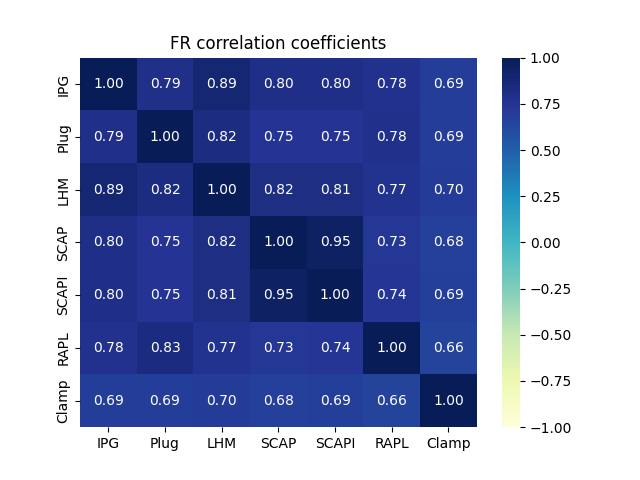
\includegraphics[width=0.6\textwidth]{figures/Fannkuch-redux_ex2.png}
    \caption{Heatmap showing the correlation coefficient between all of the measurement instruments for FR on DUT 2}
    \label{fig:fannkuchCorrDut2}
\end{figure}

All the measuring instruments showed moderate to high correlation with the ground truth (Clamp) when assessed with the Guildford Scale. On FR in \cref{fig:fannkuchCorrDut2} the software-based measuring instruments had a correlation of $0.66$ - $0.7$ while the Plug had a correlation of $0.69$. While on MB they correlations were a little lower for the software based measuring instruments as shown in \cref{app:cor_exp_two}. We expected the correlation of the software based measuring instruments to be similar since they are using the same hardware counters and MSRs. For the remaining experiments, we chose the software-based instrument based on considerations of accuracy, ease of use, and availability as expressed in \cref{RQ:RQ2}. While SCAPI had the highest correlation on both MB and FR, it and SCAP had a low sample rate and was tedious to set up on Windows, therefore it is not picked. LHM and IPG were close as IPG was slightly more correlated with the Clamp (W) on MB, but slightly less on FR. However, LHM had more problems in the setup phase than IPG and also required calculations for getting the measurements in joules, therefore, we chose IPG. %One thing to note is that our determination of accuracy is based of the accuracy of the Clamp, which means that if the Clamp is not accurate, then we do not know if the other measuring instruments are.